\section*{Aufgabe 1: \emph{Fisher--Diskriminante: Implementierung}}
\begin{itemize}
\item[a)] Die Mittelwerte der Verteilungen sind: $\vec{\mu_0} = (0.0223 ; 3.0256) $ und $\vec{\mu_1} = (5.9857 ; 3.0980)$

\item[b)] Die Streumatrix innerhalb der Klassen berechnet sich zu:
\begin{equation}
S_W = 	\begin{pmatrix} 122897.8111 & 81975.1909\\
 						81975.1909 & 67446.7286
 		\end{pmatrix} 
\end{equation}
Die Streumatrix zwischen den Klassen berechnet sich zu:
\begin{equation}
S_B = 	\begin{pmatrix}	8.8905\cdot 10^{4}  & 1.0789\cdot 10^3 \\
						1.0789\cdot 10^{3}  & 1.3092\cdot 10^1
 		\end{pmatrix} 
\end{equation}
\item[c)] Die Eigenvektoren berechnen sich zu:
\begin{align*}
\vec{\lambda_1} =& ( 0.6367 ; -0.7711 ) \quad \text{mit:}\quad \lambda_1 = 3.71 \\
\vec{\lambda_2} =& ( -0.0121 ; 0.9999 ) \quad \text{mit:}\quad \lambda_2 = 1.39 \cdot 10^{-17}
\end{align*}
\item[d)] Die Projektion der Populationen $P_0$ und $P_1$ auf die Geraden $\lambda_i$.
\begin{figure}[H]
	\centering
	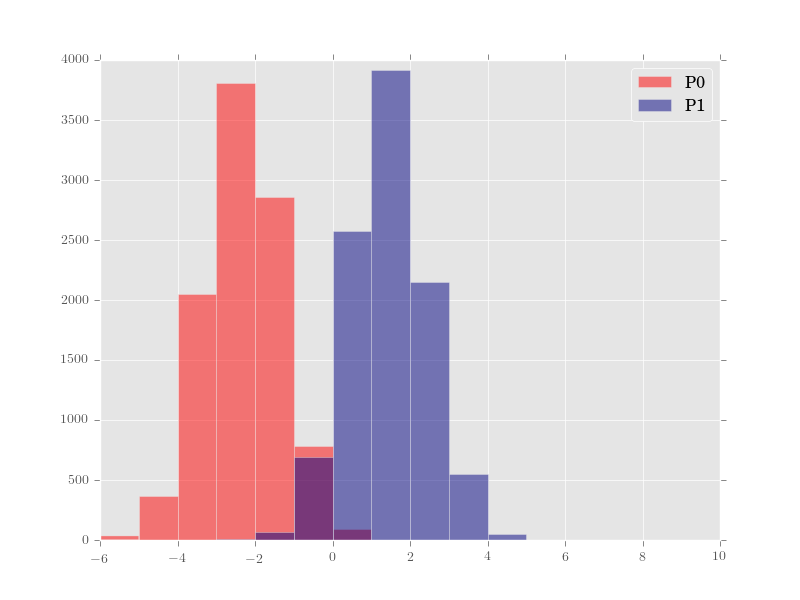
\includegraphics[width=0.7\textwidth]{hist_0.png}
	\caption{ Projektion der Populationen auf die Gerade $\lambda_1$}
\end{figure}
\begin{figure}[H]
	\centering
	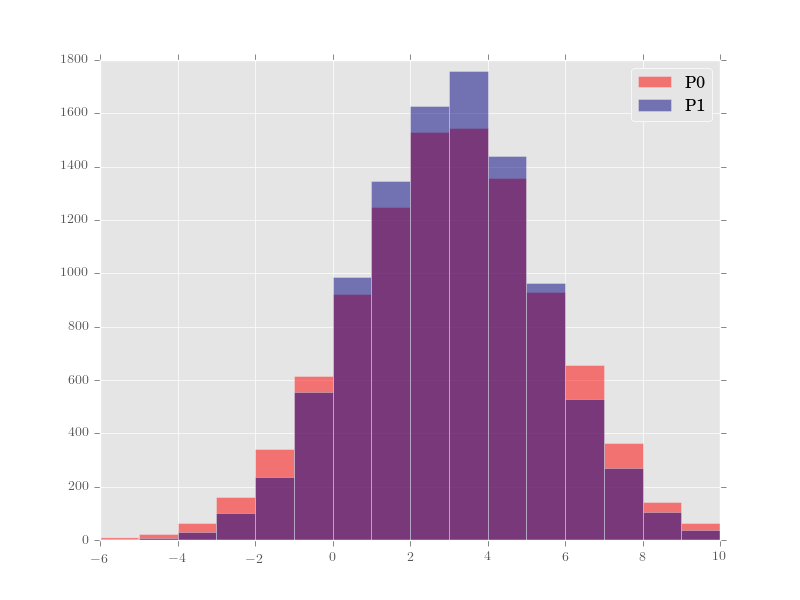
\includegraphics[width=0.7\textwidth]{hist_1.png}
	\caption{Projektion der Populationen auf die Gerade $\lambda_2$}
\end{figure}
\item[e)] Die Performanz in Abhängigkeit des gewählten Schnittes:
\begin{figure}[H]
	\centering
	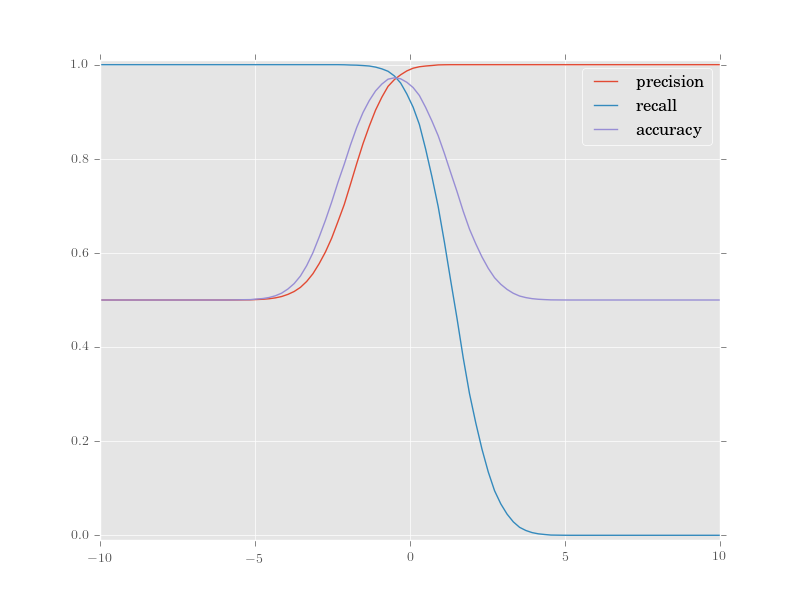
\includegraphics[width=0.7\textwidth]{performace_1.png}
	\caption{Performanz für die Projektion der Populationen auf die Gerade $\lambda_1$}
\end{figure}
\begin{figure}[H]
	\centering
	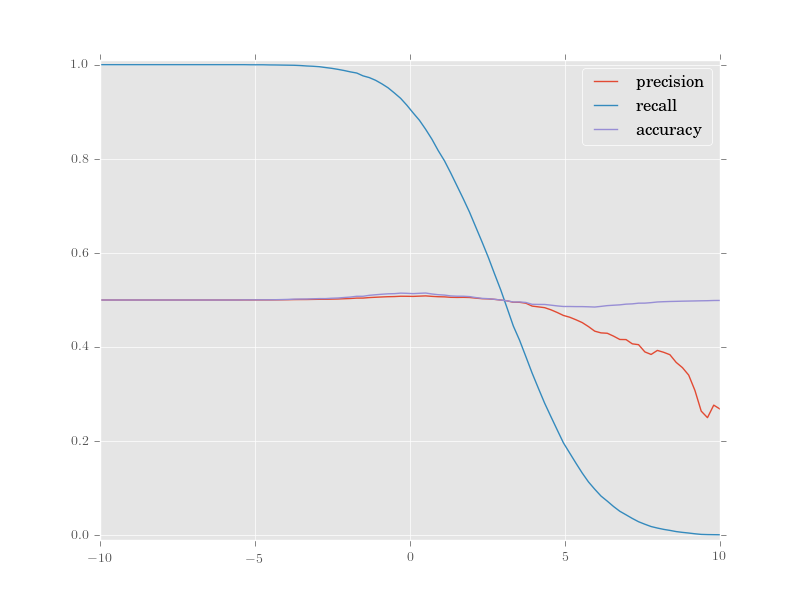
\includegraphics[width=0.7\textwidth]{performace_2.png}
	\caption{Performanz für die Projektion der Populationen auf die Gerade $\lambda_2$}
\end{figure}
\item[f)] Das Signal-Untergrundverhältnis wird für die Projektion auf $\lambda_1$ bei $\lambda_{\text{cut}}\approx -5.76$ und für die Projektion auf $\lambda_2$ bei $\lambda_{\text{cut}}\approx -5.36$ maximal.
\begin{figure}[H]
	\centering
	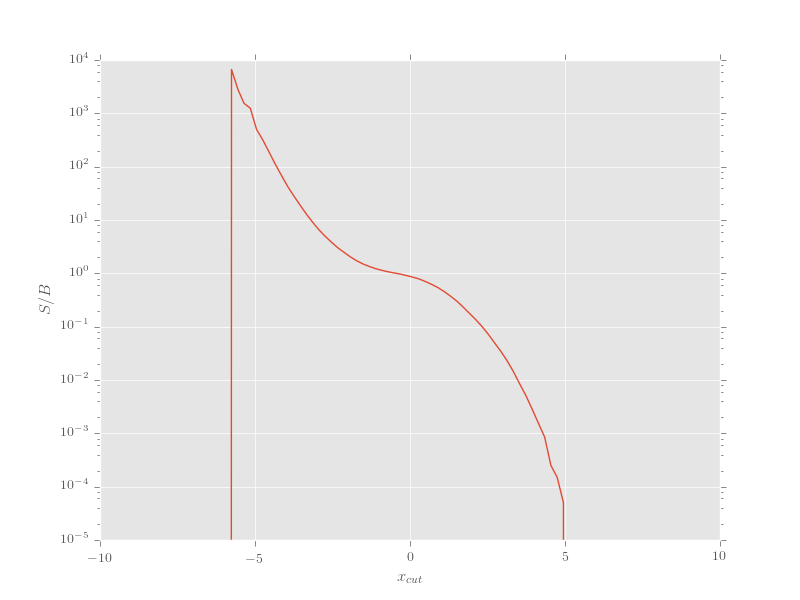
\includegraphics[width=0.7\textwidth]{sig_bkg_ratio.png}
	\caption{Signal-Untergrundverhätnis für die Projektion der Populationen auf die Gerade $\lambda_1$}
\end{figure}
\begin{figure}[H]
	\centering
	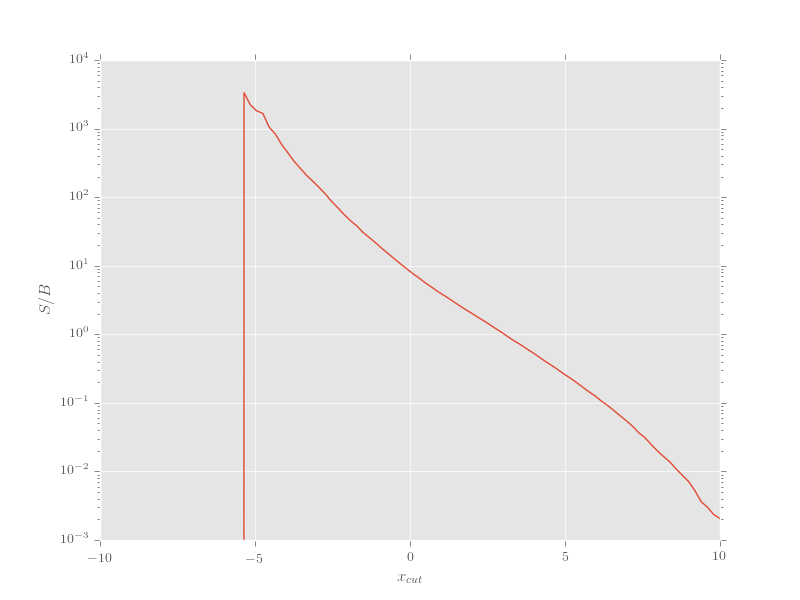
\includegraphics[width=0.7\textwidth]{sig_bkg_ratio2.png}
	\caption{Signal-Untergrundverhätnis für die Projektion der Populationen auf die Gerade $\lambda_2$}
\end{figure}

\item[g)] Die Signifikanz wird für die Projektion auf $\lambda_1$ bei $-10 \leq \lambda_{\text{cut}} \leq -5.96$ und für die Projektion auf $\lambda_2$ bei $-10 \leq \lambda_{\text{cut}} \leq -5.56$ maximal.
\begin{figure}[H]
	\centering
	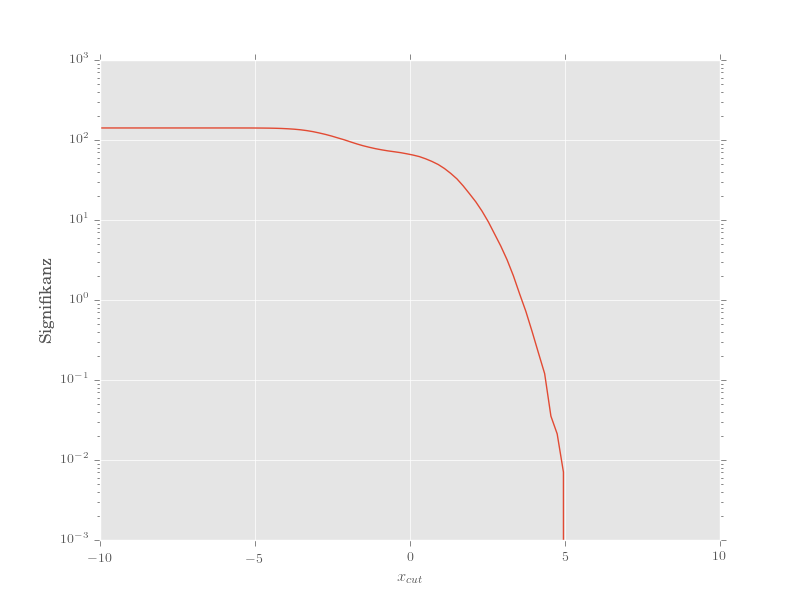
\includegraphics[width=0.7\textwidth]{signifikanz.png}
	\caption{Signifikanz für die Projektion der Populationen auf die Gerade $\lambda_1$}
\end{figure}
\begin{figure}[H]
	\centering
	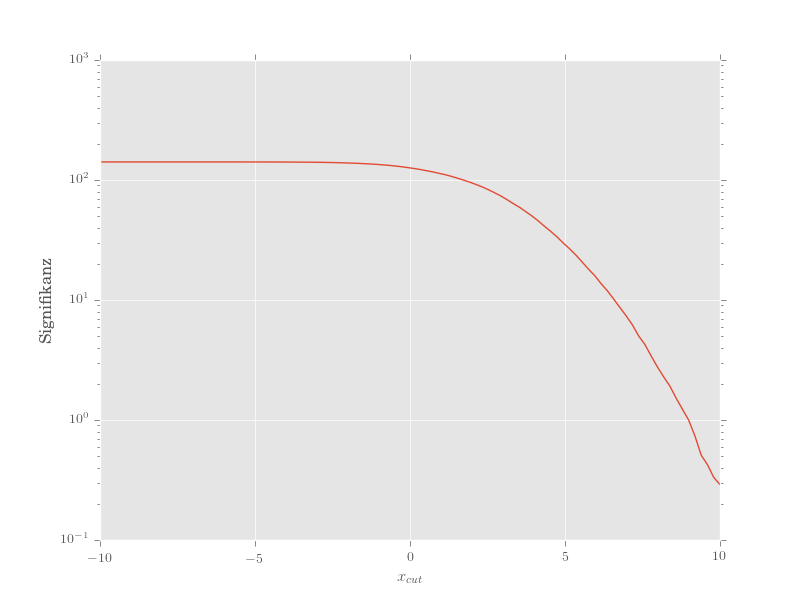
\includegraphics[width=0.7\textwidth]{signifikanz2.png}
	\caption{Signifikanz für die Projektion der Populationen auf die Gerade $\lambda_2$}
\end{figure}

\item[h)] Analog für den kleineren Datensatz von $P_0$ nur mit der Gerade $\lambda_1$.

\item[he)] Die Performanz in Abhängigkeit des gewählten Schnittes:
\begin{figure}[H]
	\centering
	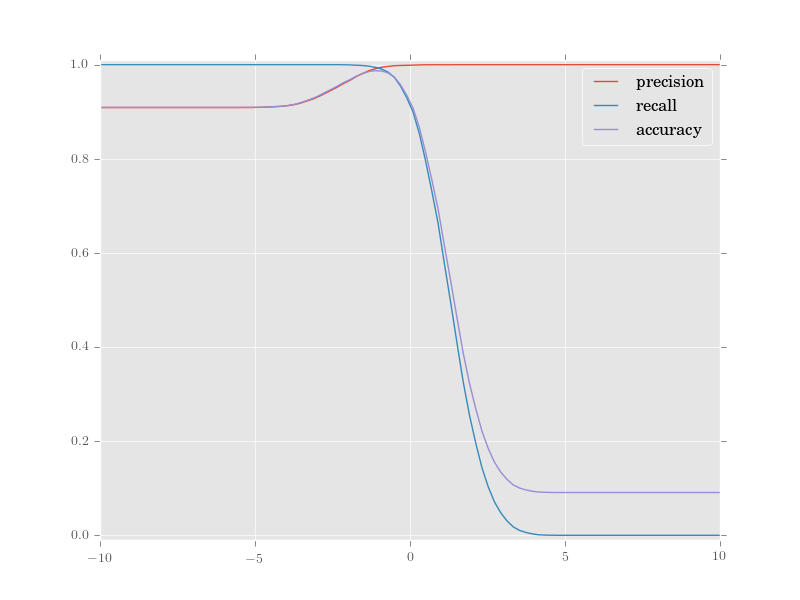
\includegraphics[width=0.7\textwidth]{performace_1_h.png}
	\caption{Performanz für die Projektion der Populationen auf die Gerade $\lambda_1$}
\end{figure}

\item[hf)] Das Signal-Untergrundverhältnis wird für die Projektion auf $\lambda_1$ bei $\lambda_{\text{cut}}\approx -5.35$maximal.
\begin{figure}[H]
	\centering
	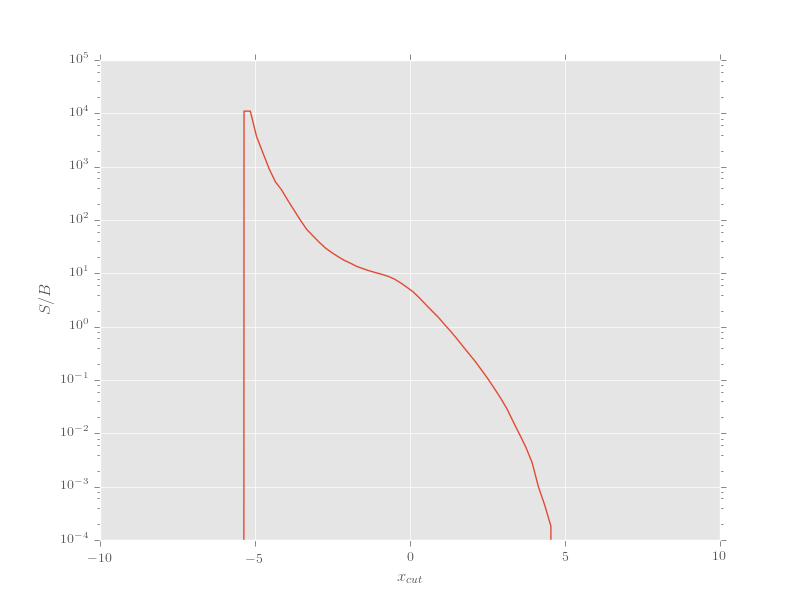
\includegraphics[width=0.7\textwidth]{sig_bkg_ratio_h.png}
	\caption{Signal-Untergrundverhätnis für die Projektion der Populationen auf die Gerade $\lambda_1$}
\end{figure}


\item[hg)] Die Signifikanz wird für die Projektion auf $\lambda_1$ bei $-10 \leq \lambda_{\text{cut}} \leq -5.55$ maximal.
\begin{figure}[H]
	\centering
	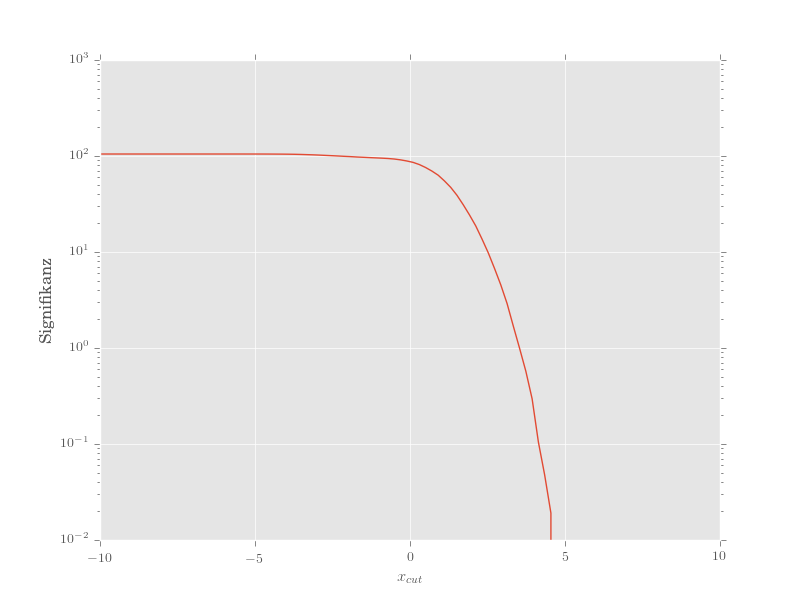
\includegraphics[width=0.7\textwidth]{signifikanz_h.png}
	\caption{Signifikanz für die Projektion der Populationen auf die Gerade $\lambda_1$}
\end{figure}



\end{itemize}
\section*{Aufgabe 2: \emph{kMeans per Hand}}

Population: $(1,4) (1,5) (1,6) (3,3) (3,2) (4,1) (5,1) (6,2) (6,3) (8,4) (8,5) (8,6)$\\
Clusterzentren: $(3,4) (7,4) (3,7)$

\begin{table}
\centering
\caption{Zu den ursprünglich gewählten Clusterzentren gehörende Datenpunkte.}
\begin{tabular}{S S S S S S S}
\toprule
\multicolumn{1}{c}{Clusterzentrum} & \multicolumn{6}{c}{Datenpunkte} \\
\midrule
\text{(3.00, 4.00)}& \text{(1,5)} &\text{(1,4)}& \text{(3,3)}& \text{(3,2)} &\text{(4,1)}& \\
\text{(7.00, 4.00)}& \text{(6,2)} &\text{(6,3)} &\text{(8,4)} &\text{(8,5)}& \text{(8,6)} &\text{(5,1)}\\
\text{(3.00, 7.00)}& \text{(1,6)} &&&&&\\
\bottomrule
\end{tabular}
\end{table}

\begin{table}
\centering
\caption{Berechnete Clusterzentren nach der ersten Iteration und Zugehörigkeit der Datenpunkte.}
\begin{tabular}{S S S S S S S S}
\toprule
\multicolumn{1}{c}{Clusterzentrum} & \multicolumn{6}{c}{Datenpunkte} \\
\midrule
\text{(2.40, 3.00)}        &\text{(1,4)}& \text{(3,3)} & \text{(3,2)}& \text{(4,1)}&& \\
\text{(6.83, 3.50)}&\text{(5,1)}& \text{(6,2)}&\text{(6,3)}&\text{(8,4)}&\text{(8,5)}&\text{(8,6)} \\
\text{(1.00, 6.00) }           &\text{(1,6)}& \text{(1,5)}&&&&\\
\bottomrule
\end{tabular}
\end{table}

\begin{table}
\centering
\caption{Berechnete Clusterzentren nach der zweiten Iteration und Zugehörigkeit der Datenpunkte.}
\begin{tabular}{S S S S S S S S}
\toprule
\multicolumn{1}{c}{Clusterzentrum} & \multicolumn{6}{c}{Datenpunkte} \\
\midrule
\text{(2.75, 2.50)}        &\text{(5,1)}& \text{(3,3)} & \text{(3,2)}& \text{(4,1)}&& \\
\text{(6.83, 3.50)}&\text{(6,2)}&\text{(6,3)}&\text{(8,4)}&\text{(8,5)}&\text{(8,6)}& \\
\text{(1.00, 5.50) }           &\text{(1,6)}& \text{(1,5)}&\text{(1,4)}&&&\\
\bottomrule
\end{tabular}
\end{table}

\begin{table}
\centering
\caption{Berechnete Clusterzentren nach der dritten Iteration und Zugehörigkeit der Datenpunkte.}
\begin{tabular}{S S S S S S S S}
\toprule
\multicolumn{1}{c}{Clusterzentrum} & \multicolumn{6}{c}{Datenpunkte} \\
\midrule
\text{(3.75, 1.75)}        &\text{(5,1)}& \text{(3,3)} & \text{(3,2)}& \text{(4,1)}&\text{(6,2)}& \\
\text{(7.20, 4.00)}&\text{(6,3)}&\text{(8,4)}&\text{(8,5)}&\text{(8,6)}&& \\
\text{(1.00, 5.00) }           &\text{(1,6)}& \text{(1,5)}&\text{(1,4)}&&&\\
\bottomrule
\end{tabular}
\end{table}

\begin{table}
\centering
\caption{Berechnete Clusterzentren nach der vierten Iteration und Zugehörigkeit der Datenpunkte.}
\begin{tabular}{S S S S S S S S}
\toprule
\multicolumn{1}{c}{Clusterzentrum} & \multicolumn{6}{c}{Datenpunkte} \\
\midrule
\text{(4.20, 1.80)}        &\text{(5,1)}& \text{(3,3)} & \text{(3,2)}& \text{(4,1)}&\text{(6,2)}& \\
\text{(7.50, 4.50)}&\text{(6,3)}&\text{(8,4)}&\text{(8,5)}&\text{(8,6)}&& \\
\text{(1.00, 5.00) }           &\text{(1,6)}& \text{(1,5)}&\text{(1,4)}&&&\\
\bottomrule
\end{tabular}
\end{table}


\begin{table}
\centering
\caption{Berechnete Clusterzentren nach der fünften Iteration und Zugehörigkeit der Datenpunkte.}
\begin{tabular}{S S S S S S S S}
\toprule
\multicolumn{1}{c}{Clusterzentrum} & \multicolumn{6}{c}{Datenpunkte} \\
\midrule
\text{(4.20, 1.80)}        &\text{(5,1)}& \text{(3,3)} & \text{(3,2)}& \text{(4,1)}&\text{(6,2)}& \\
\text{(7.50, 4.50)}&\text{(6,3)}&\text{(8,4)}&\text{(8,5)}&\text{(8,6)}&& \\
\text{(1.00, 5.00) }           &\text{(1,6)}& \text{(1,5)}&\text{(1,4)}&&&\\
\bottomrule
\end{tabular}
\end{table}

\begin{figure}[H]
	\centering
	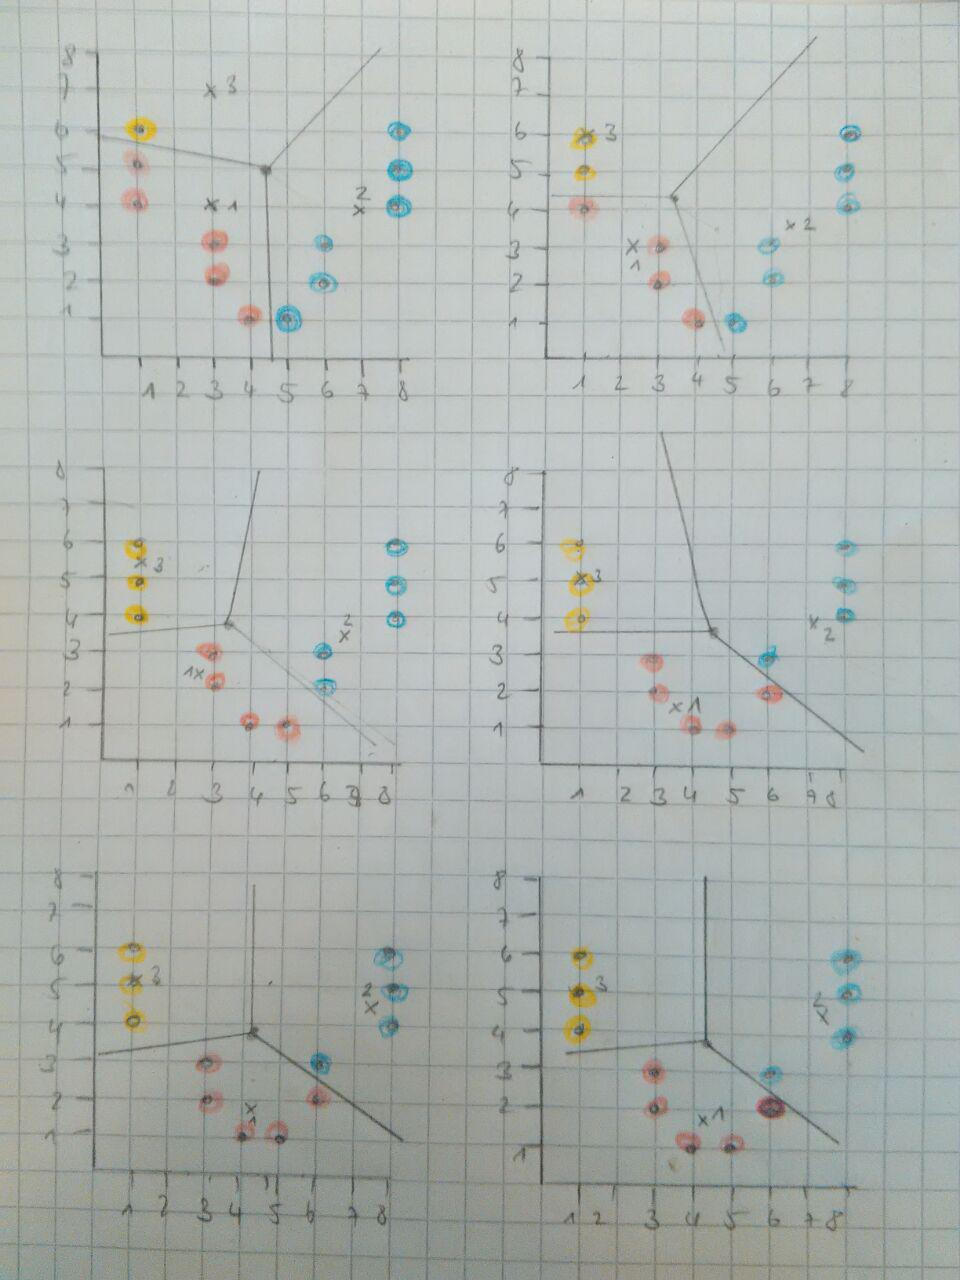
\includegraphics[width=0.7\textwidth]{kmeans.jpg}
	\caption{Zugehörigkeit der Datenpunkte zu den Clusterzentren nach jeder Iteration.}
\end{figure}



Die Berechnung der Abstände einiger Punkte zu den Clustern, die Berechnung der neuen Clusterzentren als Mittelwert ihrer zugehörigen Datenpunkte und die Berechnung der Clustergrenzen sind nicht mit aufgeführt. \newline
Die Verteilung der Datenpunkte auf die drei Clustern ändert sich zwischen der vierten und fünften Iteration nicht; der Algorithmus konvergiert. \newline
Die Verteilung der Punkte auf die Zentren entspricht der intuitiven Gruppierung der Punkte bei Betrachtung der Abbildung. Nur den Punkt $(6,3)$ würde man eher zu Cluster $1$ zählen; laut Algorithmus gehört er jedoch zu Cluster $2$.


\section*{Aufgabe 3: \emph{Feature Selection mit dem MRMR--Algorthmus}}
\begin{itemize}
\item[a), b) und c)]
\end{itemize}
\begin{figure}[H]
	\centering
	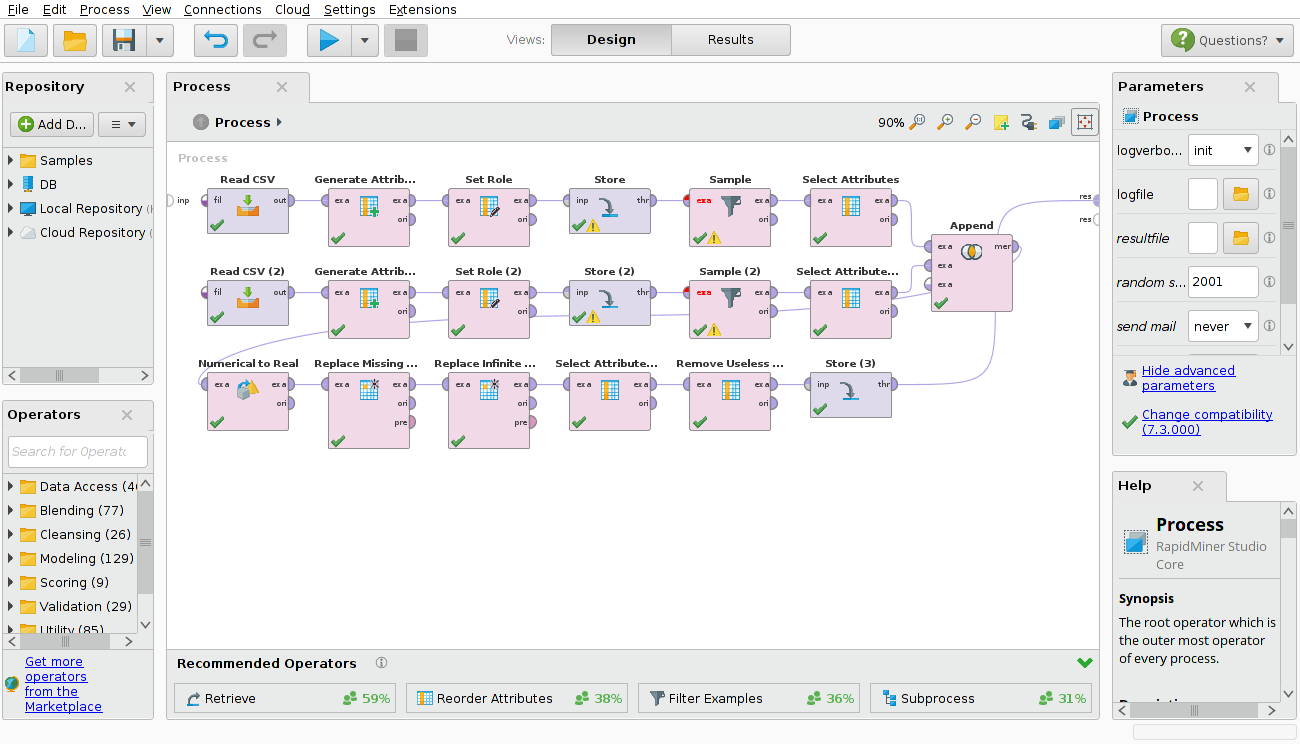
\includegraphics[width=0.9\textwidth]{Rapidminer/Datenbereinigung.png}
	\caption{Reduktion der Datensätze auf insgesamt $4000$ Ereignisse. Anschließend werden die Daten bereinigt, indem einige Attribute, zum Beispiel wegen fehlender Werte, entfernt werden. Ein \emph{label} wird vergeben, um Signal und Untergrund voneinander unterscheiden zu können.}
\end{figure}

\begin{figure}[H]
	\centering
	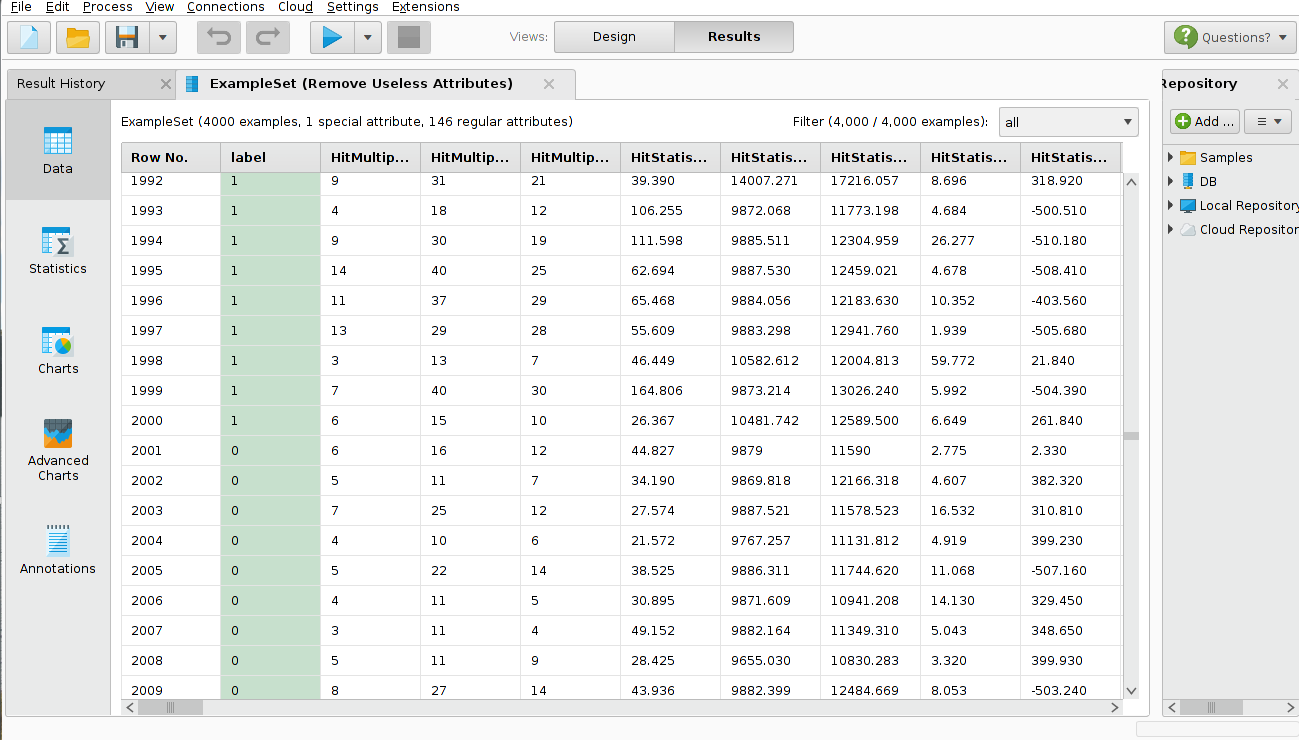
\includegraphics[width=0.9\textwidth]{Rapidminer/Datenbereinigung_2.png}
	\caption{Ergebnisse der Datenbereinigung. Es sind $4000$ Ereignisse mit $146$ regulären und einem speziellen Attribut übrig. Dabei wurde unter anderem der für Aufgabe b) benötigte Operator "Remove Useless Attributes" benutzt.}
\end{figure}

\begin{figure}
	\centering
	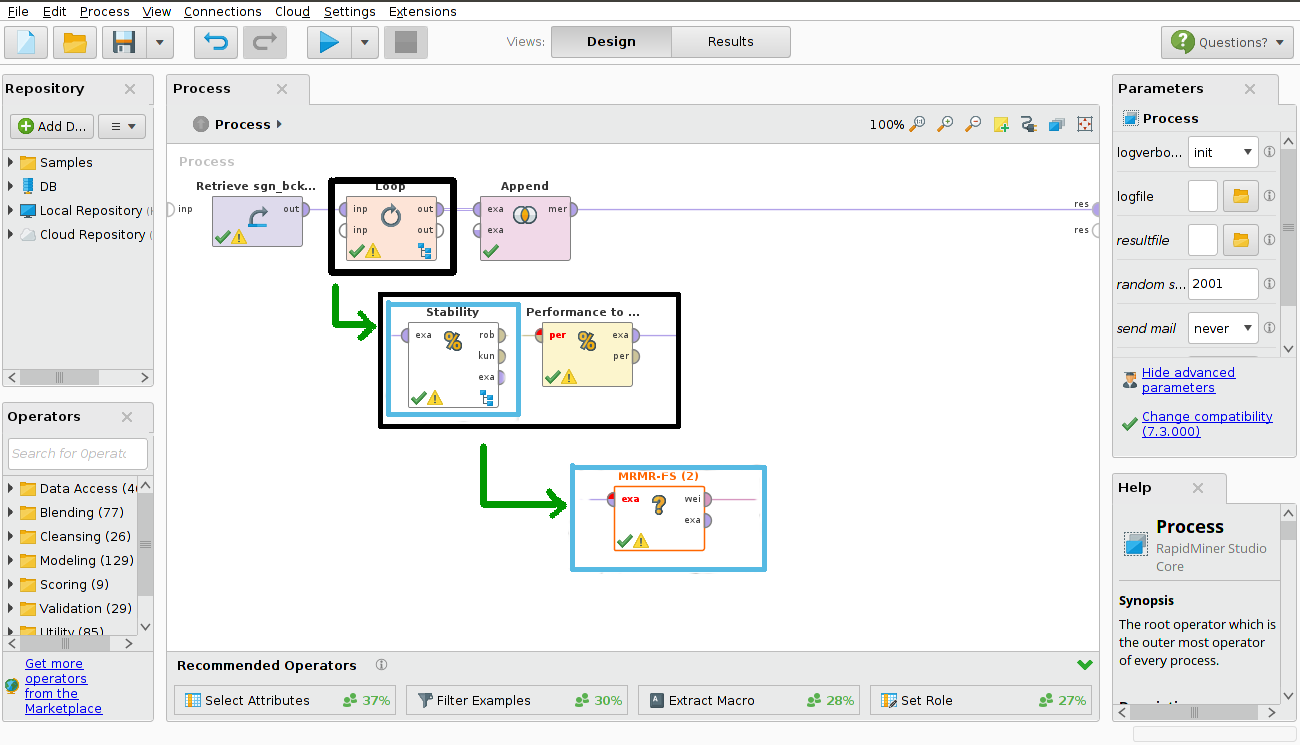
\includegraphics[width=0.9\textwidth]{Rapidminer/Zusammenfassung.png}
	\caption{Prozess zur Erstellung eines Plots für die Stabilität der Attributsauswahl.}
\end{figure}

\begin{figure}
	\centering
	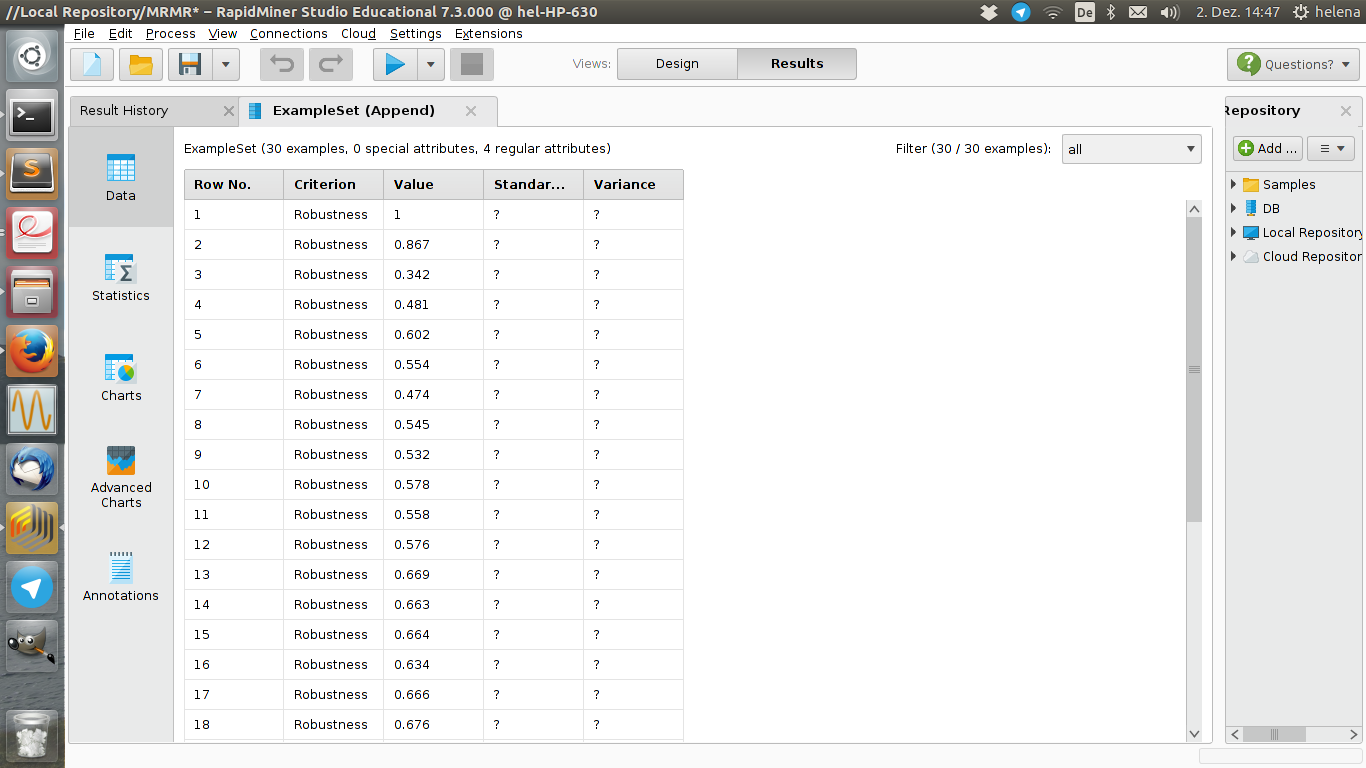
\includegraphics[width=0.9\textwidth]{Rapidminer/MRMR_results.png}
	\caption{ Projektion der Populationen auf die Gerade $\lambda_1$}
\end{figure}

\begin{figure}
	\centering
	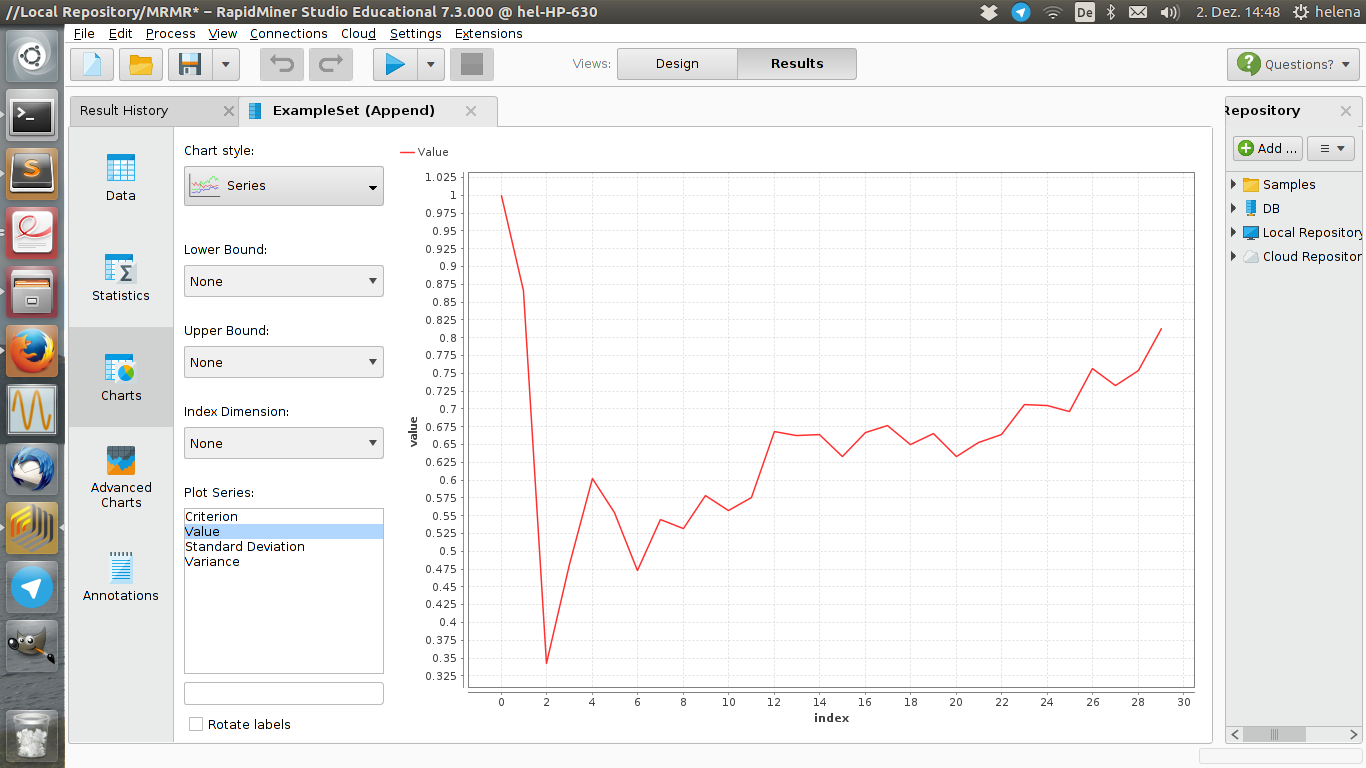
\includegraphics[width=0.9\textwidth]{Rapidminer/Plot.png}
	\caption{Darstellung der Stabilität der zuvor getätigten Attributsauswahl.}
\end{figure}